\documentclass[xetex,mathsans,sans,aspectratio=169]{beamer}
\usepackage{listings}
\usetheme{Boadilla}
\usecolortheme{orchid}
\usepackage{fontspec}
\setsansfont{Basis Grotesque}
\setbeamertemplate{navigation symbols}{}
\usepackage{amsmath}
\usepackage{multicol}

% The title slide information about the presenter(s) eg. name(s), role(s)
\newcommand{\presenter}{<presenter name(s), role(s)>}

% The text for the presenter footer eg. first name(s)
\newcommand{\presenterfooter}{<presenter fname(s)>}

% The footer title of the presentation (optional - default is 'NuCypher')
\newcommand{\titlefooter}{NuCypher}

% The email name prefix for the presenter i.e. <email_prefix>@nucypher.com
\newcommand{\emailname}{<email\_prefix>}

% The name of the event
\newcommand{\event}{<event name>}

% The date of the event with format: dd MMM yyyy
\newcommand{\eventdate}{<dd MMM yyyy>}


% Example usage:
%
%     \newcommand{\presenter}{MacLane Wilkison, CEO \& Co-Founder}
%     \newcommand{\presenterfooter}{MacLane}
%     \newcommand{\titlefooter}{NuCypher}
%     \newcommand{\emailname}{maclane}
%     \newcommand{\event}{Eth SF}
%     \newcommand{\eventdate}{05 Oct 2018}
%


\title[\titlefooter]{Decentralized internet: beyond public key encryption

\includegraphics[width=5.5cm]{pdf/nucypher_logo.pdf}}
\author[\presenterfooter]{\presenter}
\date[\eventdate]{\event, \eventdate}

\begin{document}
    \begin{frame}
        \titlepage
    \end{frame}

    \begin{frame}
        \frametitle{Transport encryption in traditional internet}
        \begin{figure}
            \centering
            \includegraphics<1>[width=\textwidth]{pdf/file-sharing-tls.pdf}\includegraphics<2>[width=\textwidth]{pdf/file-sharing-tls-danger.pdf}
        \end{figure}
    \end{frame}

    \begin{frame}
        \frametitle{Does TLS work when decentralized?}
        \begin{figure}
            \centering
            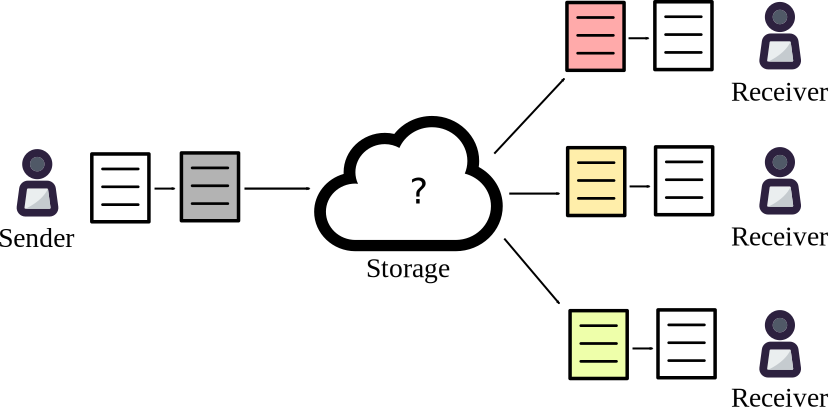
\includegraphics[width=\textwidth]{pdf/file-sharing.pdf}
        \end{figure}
    \end{frame}

    \begin{frame}
        \frametitle{Proxy re-encryption (PRE)}
        \begin{figure}
            \centering
            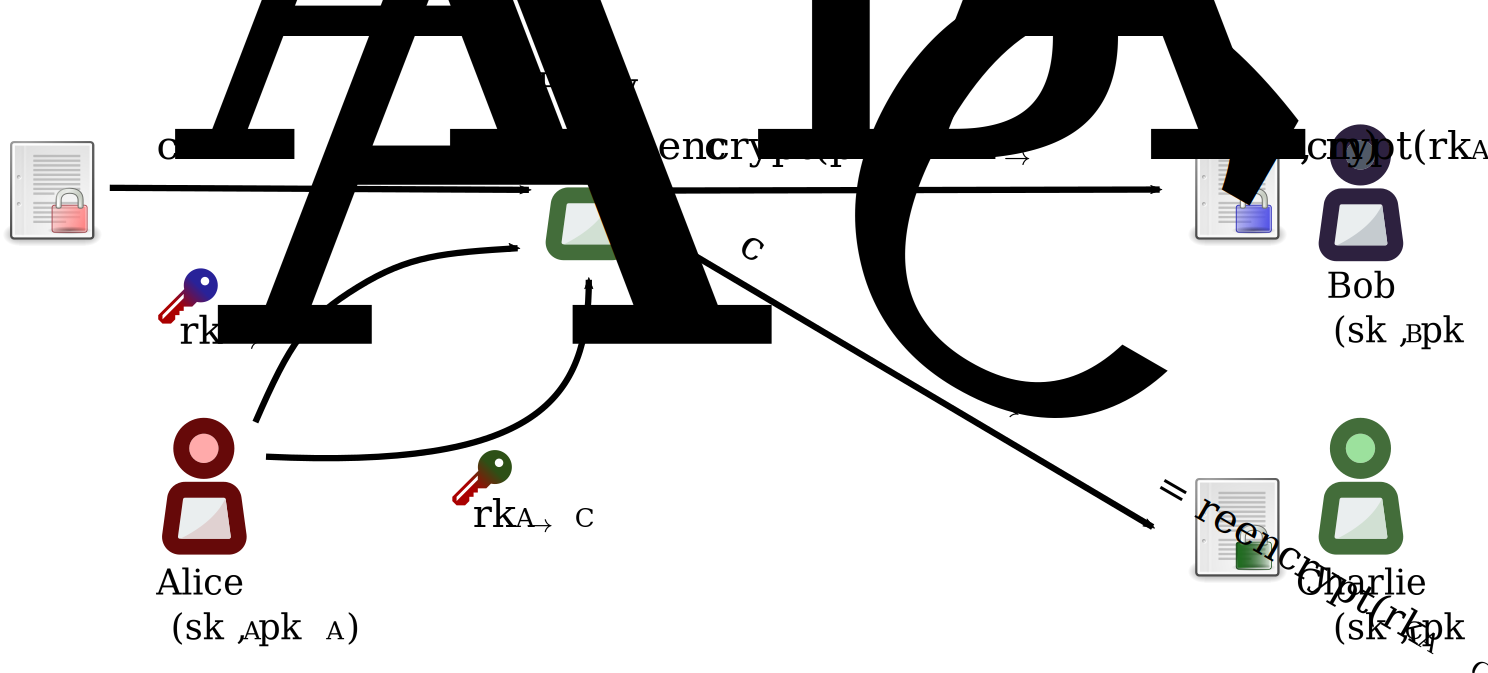
\includegraphics[width=\textwidth]{pdf/pre-multi.pdf}
        \end{figure}
    \end{frame}

    \begin{frame}
        \frametitle{Decentralized permission management via PRE}
        \begin{figure}
            \centering
            \includegraphics<1>[height=0.6\textheight]{pdf/delegate.pdf}\includegraphics<2>[height=0.6\textheight]{pdf/encrypt.pdf}\includegraphics<3>[height=0.6\textheight]{pdf/decrypt.pdf}\includegraphics<4>[height=0.6\textheight]{pdf/pre-kms.pdf}
        \end{figure}
    \end{frame}

    \begin{frame}
        \frametitle{Umbral: Threshold Proxy Re-encryption}
        \begin{figure}
            \centering
            \includegraphics[width=11cm]{pdf/umbral-kem-flow.pdf}
        \end{figure}
        \begin{itemize}
            \item Reference implementation: \url{https://github.com/nucypher/pyUmbral}
            \item Documentation: \url{https://github.com/nucypher/umbral-doc}
        \end{itemize}
    \end{frame}

    \begin{frame}
        \frametitle{Umbral: Threshold Proxy Re-encryption}
        \begin{itemize}
        	\item \emph{``Umbral''} is Spanish for \emph{``threshold''}
            \item PRE properties: Unidirectional, single-hop, non-interactive
            \item Follows a KEM/DEM approach:
            	\begin{itemize}
		    \item UmbralKEM provides the threshold re-encryption capability
                    \item Uses ECIES for key encapsulation with ZK proofs of correctness for verifiability on prime order curves (such as secp256k1)
            	    \item DEM can be any authenticated encryption (currently ChaCha20-Poly1305)
        	\end{itemize}
	    \item IND-PRE-CCA security
            \item Key splitting is analogous to Shamir Secret Sharing
	    \item Verification of re-encryption correctness through Non-Interactive ZK Proofs
            \item Reference implementation: \url{https://github.com/nucypher/pyUmbral}
	    \item Documentation: \url{https://github.com/nucypher/umbral-doc}
        \end{itemize}
    \end{frame}

    \begin{frame}
        \frametitle{How to go beyond sharing}
        Multi-Party Computation
        \begin{itemize}
           \item Interactive protocol
           \item Slow Performance
        \end{itemize}

        Fully Homomorphic Encryption
        \begin{itemize}
           \item Slow Peformance
           \begin{itemize}
               \item NuCypher has developed a GPU-accelerated FHE library: nuFHE
           \end{itemize}
        \end{itemize}

        Non-interactive Zero-Knowledge proofs
        \begin{itemize}
            \item Actively researched now
            \item Useful even beyond privacy-preserving value transfers
        \end{itemize}

        Oblivious RAMs
        \begin{itemize}
            \item For hiding access patterns
            \item Didn't receive much of attention by DApps yet
        \end{itemize}
    \end{frame}

    \begin{frame}
      \frametitle{Fully Homomorphic Encryption}
       \framesubtitle{nuFHE library}
       \begin{itemize}
           \item Based on TFHE: Fast Fully Homomorphic Encryption over the Torus
           \item GitHub: \url{https://github.com/nucypher/nufhe}
           \item GPU implementation of fully homomorphic encryption
           \item Uses either FFT or integer NTT
           \item Achieved 100x performance over TFHE benchmarks
           \begin{figure}
               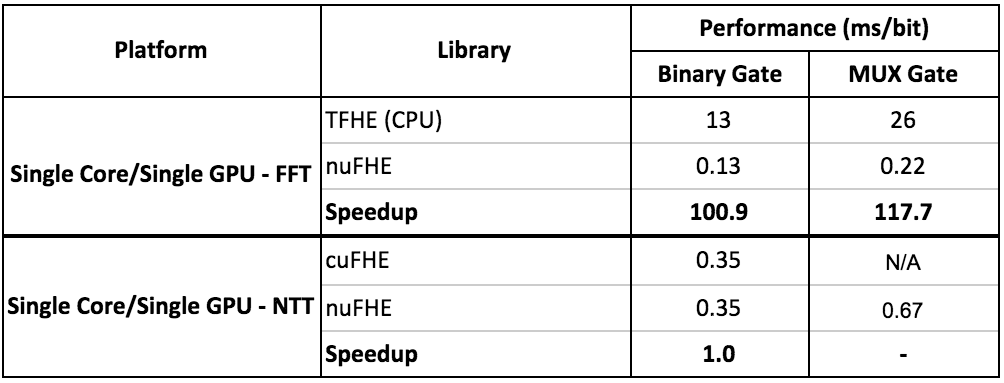
\includegraphics[width=10.5cm]{pdf/nufhe-benchmarks.pdf}
           \end{figure}
       \end{itemize}
     \end{frame}

    \begin{frame}
      \frametitle{FHE Proof of Concept}
      \framesubtitle{Sputnik}
      \begin{itemize}
        \item GitHub: \url{https://github.com/nucypher/sputnik}
        \item Assembly language and interpreter for FHE that uses nuFHE
        \item Commits a merkle root of computation to the blockchain for proof of logic flow
        \item Used to execute first homomorphic smart contract at ETHBerlin 2018
      \end{itemize}
      \begin{figure}
        \centering
        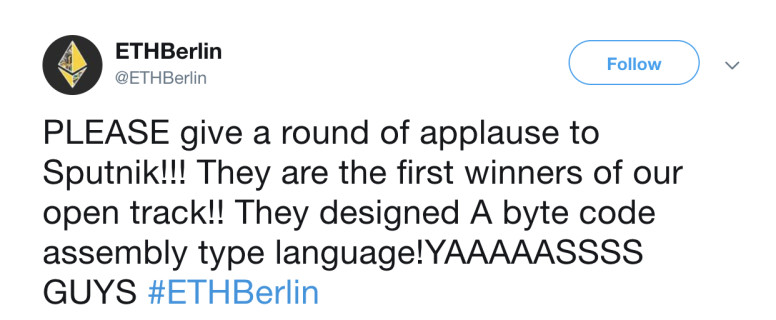
\includegraphics[width=8cm]{pdf/sputnik-tweet.pdf}
      \end{figure}
    \end{frame}

    \begin{frame}
        \frametitle{Can DApps propel privacy-preserving computations\\
        research and adoption?}
        \begin{itemize}
            \item CPU: $70$ ops/s;
            \item GPGPU: $7000$ ops/s;
            \item FPGA: ???;
            \item ASIC: 1M ops/s?;
            \item Optical computers: on par with CPUs while keeping data encrypted?
            \begin{itemize}
                \item Hint: a thin lens can do FFT
            \end{itemize}
        \end{itemize}
    \end{frame}

    \begin{frame}
        \frametitle{Conclusion and references}
        \begin{figure}
            \centering
            
\includegraphics[width=3cm]{pdf/nucypher_logo.pdf}
        \end{figure}
        Website: \url{https://www.nucypher.com}

        Whitepaper: \url{https://www.nucypher.com/whitepapers/english.pdf}

        Proxy Re-encryption Network: \url{https://github.com/nucypher/nucypher}

        Umbral Reference Implementation: \url{https://github.com/nucypher/pyUmbral}

        nuFHE: \url{https://github.com/nucypher/nufhe}

        Discord: \url{https://discord.gg/7rmXa3S}

        E-mail: \href{mailto:\emailname @nucypher.com}{\emailname @nucypher.com}

        E-mail: \href{mailto:hello@nucypher.com}{hello@nucypher.com}
    \end{frame}
\end{document}

